\documentclass[11pt]{article}
\usepackage[margin=1.1in]{geometry}
\usepackage{amsmath,amssymb,amsthm}
\usepackage{booktabs}
\usepackage{array}
\usepackage{tabularx}
\usepackage[protrusion=true,expansion=false]{microtype}
\usepackage[table]{xcolor}
\usepackage{enumitem}
\usepackage{titlesec}
\usepackage{tikz}
\usepackage{float}
\usetikzlibrary{arrows.meta,positioning,fit,calc,decorations.pathreplacing}
\usepackage{listings}
\usepackage{hyperref}

\hypersetup{colorlinks=true, linkcolor=blue!60!black, urlcolor=blue!60!black, citecolor=blue!60!black}
\usepackage[skip=0.6\baselineskip, indent=0pt]{parskip}

\titleformat{\section}{\large\bfseries}{\thesection.}{0.7em}{}
\titleformat{\subsection}{\normalsize\bfseries}{\thesubsection.}{0.6em}{}

\newcommand{\vmax}{V_{\max}}
\newcommand{\Tc}{T_{\mathrm{close}}}
\newcommand{\tx}[1]{\texttt{#1}}
\newcolumntype{L}{>{\raggedright\arraybackslash}X}

\lstdefinestyle{script}{
  basicstyle=\ttfamily\small,
  columns=fullflexible,
  keepspaces=true,
  breaklines=true,
  frame=single,
  framerule=0.3pt,
  xleftmargin=1em,
  escapeinside={(*}{*)},
}

\newtheorem{assumption}{Assumption}

% tables: a little more room between rows, and every other row shaded, so
% that rows of wrapped text stay distinct
\renewcommand{\arraystretch}{1.3}
\rowcolors{1}{}{black!5}

\definecolor{coop}{RGB}{232,245,233}
\definecolor{chainc}{RGB}{255,228,225}
\definecolor{proofc}{RGB}{230,240,255}

\title{\textbf{Lichen}\\L2s In CHannels ENforced by bitcoin}
\author{waxwing}
\date{Version 0.2, October 2026}

\begin{document}
\maketitle

\begin{abstract}
A \emph{contract} with a hub lets a user hold the hub's tokens on a layer 2 and
withdraw them as bitcoin without trusting the hub for honesty or liveness. The L2 tokens are collateralised by the bitcoin in the user-hub multisig output\footnote{a standalone 2-of-2 output (a channel embedding is possible; Section~\ref{sec:contract})}, and if the hub refuses a withdrawal, or cannot answer because it is offline, it is enforced on Bitcoin. The only assumptions are those of the layer 2 itself, kept apart from the hub. No change to Bitcoin's
consensus is required. A withdrawal is a claim that a program, the withdrawal statement, ran on some input and produced an output: the statement is proved with RISC Zero and wrapped in Groth16, and a disputed claim is settled on Bitcoin by verification of the Groth16 proof.  Withdrawals are executed cooperatively in the contract --- with overwhelming likeliness because the statement is deterministically verifiable in milliseconds --- or, otherwise, a refused one is played as dispute on-chain over the verifier, with this dispute having been set up at the start of each contract. The trustlessness gain is paid for with liquidity (with receiving ability only contingent on offered ``inbound'' from the hub, as in Lightning). The hub (but not user) must also stay live during normal operation, since an offline hub loses disputes by timeout. The design, including a privacy-focused shielded note L2, is built and measured in~\cite{lichencode}.
\end{abstract}

\tableofcontents

\section{Introduction}

\subsection{Obvious objections to Lichen and why they're mostly wrong}

\paragraph{One central hub is dangerous.} If the hub disappears, the user gets the money. The hub cannot Sybil attack users by printing tokens fictitiously; the honest users' money is all backed. The only remaining risks are inherent to the L2 itself (is it a validity rollup or a quorum? Does it inherit finality from Bitcoin or is finality weaker? Etc.)

\paragraph{Bridges usually mean you can only withdraw a fixed size utxo, meaning operators and relying on swaps. Surely that applies here?} No. The withdrawal amount is encoded in bits in the bitcoin transaction witness, in dispute. This allows us to withdraw arbitrary amounts via multiple outputs of certain denominations~[\ref{sec:outcomes}].

\paragraph{Don't these constructions usually require a 1 of n honesty assumption from a signing committee?} Not here: we avoid this by the LN-GAP~\cite{lngap} trick: the contract is a \emph{bilateral} contract between the hub and each user; the presigning happens between them, just as in Lightning.

\paragraph{But if a bunch of users open contract with a hub, they can just .. pay each other through Lightning channels?} A correct critique, partly, \underline{if} the L2 ledger doesn't do anything but plain payments. Even then, you could avoid receiver liveness being needed, avoid routing and other minor things. But the real answer is: the L2 can offer more functionality. It can use zcash style shielded notes, allowing very high privacy while staying in the L2. It can also (in a different ``lichen'' on a different hub) offer rich smart contracting, etc.

\paragraph{But this is an IOU/ hub's token, so it's not actually bitcoin.} Incorrect with a crucial caveat. See the first point: every sat is redeemable via the user-hub contracts, \emph{without} the hub's permission, one-to-one, so these are actually bitcoin \emph{but only as long as you have liquidity to receive them}. A new user on L2 without a contract with the hub, or a user holding a balance on L2 far in excess of their inbound liquidity in their own contract, is holding \emph{credit}, and has no such guarantee. But that's their choice.

\paragraph{But still, a single central hub feels like bad design. Why not multiple hubs?} Having multiple hubs \emph{will} make sense --- see Section~\ref{sec:multihub}, but done naively, it is broken. It's because of what these L2 tokens are. They are fungible, \underline{enforceable} claims on the hub's money; they are minted by the hub itself, just on its own say-so. If you had hub 1 and hub 2, those claims are not transferrable trustlessly to the hubs themselves. If hub 2 prints a billion sats out of nothing and users accept it on the L2 they can redeem it with hub1, leaving hub1 out of pocket. From this line of thinking we see an interesting comparison with ecash servers: the hub can print as much as it likes, but it cannot steal/``rug''.

\paragraph{So what's the catch?} The negatives are twofold: one is liquidity, and this is easy to understand as the analog of the inbound liquidity pain point in Lightning, because it's basically the same thing. Such a hub \emph{can} choose to give no inbound liquidity to a user: they get tokens on L2 to spend, but they cannot (safely) receive. If they receive, it's just credit that someone else will hopefully buy from them. But the design does not assume that, of course, it allows receiving up to a ``cap'': the user negotiates that extra potential receiving amount (inbound liquidity) when it sets up the contract with the hub. The second is the on-chain dispute, whose size depends on the gadget: tens of transactions and 100–200 kvB under BitVMX as built, a handful and about 30 kvB under BABE (estimated)~\cite{lichenbitvmx,lichenbabe}.

\subsection{A note on the delta to LN-GAP}
\label{sec:family}

LN-GAP~\cite{lngap} puts contracts governed by arbitrary programs into Lightning~\cite{lightning}
channels: a contract's outcome is decided by a game whose moves are
signed off-chain, with pre-signed transactions that let either party
take a dispute to Bitcoin~\cite{lngap}. Lichen mainly differs in trying to achieve trustlessness at the expense of a potentially larger (though still O(1) in the size of the withdrawal statement) onchain resolution; a tradeoff that fits well with the intent of creating \emph{an L2 from a bunch of contracts with a hub}:

\begin{center}
\small
\begin{tabularx}{\linewidth}{p{24mm}LL}
\toprule
& LN-GAP &  Lichen w/ BitVMX  \\
\midrule
venue & trusted: a majority of members attests moves & none \\
a dispute is decided by & the venue's attestations  & the chain: BitVMX's search \\
suited to & interactive games where time has value  & withdrawals from a hub's layer 2 \\
on-chain cost of a dispute & constant & log(length of Groth16 verifier program) \\
\bottomrule
\end{tabularx}
\end{center}

\paragraph{Why Lichen needs no venue.}  It's more about choice than logical requirement. In LN-GAP the parties \emph{could} just play ForceMove and accept that the game goes onchain when someone is not cooperative. That's not much fun for a 100 move chess game or similar. However the tradeoff of trust vs length of game is drastically different for Lichen: the game length is fixed in advance and might even be concretely very short using BABE rather than BitVMX. While for such an L2 to be viable it's absolutely crucial to try to remove third party trust. That's why the ``venue'' concept is removed here.

\section{Contracts with the hub}
\label{sec:terms}

\textbf{Alice}, the user, has a contract with a \textbf{Hub}, instantiated as a 2 of 2 output  (see Section~\ref{sec:contract} for the possibility of embedding this inside a Lightning channel), with these terms:
\begin{center}
\small
\begin{tabularx}{\linewidth}{p{16mm}L}
\toprule
$D$ & Alice's deposit: she puts $D$ bitcoin in and receives $D$ of the hub's tokens on the L2 \\
$\vmax$ & the most she can withdraw: her $D$ and the hub's liquidity $\vmax - D$ \\
$r_A, r_H$ & the \emph{contract reserves}, Alice's and the hub's: returned in every honest outcome, forfeited to the other side by losing a dispute (Section~\ref{sec:outcomes}); the contract holds $\vmax + r_A + r_H$ \\
$b$ & the amount she withdraws, by returning $b$ tokens to the hub on the L2 with the memo $c$ \\
$c$ & the contract's identifier, its memo \\
$\Tc$ & the contract's end: with no withdrawal by then, the hub takes it \\
\bottomrule
\end{tabularx}
\end{center}
Every token is a liability of the hub, collateralised by the contract of whoever holds it, within that holder's cap; within $\vmax$ and before $\Tc$, Alice trusts the hub for nothing, not even to be online: a withdrawal it does not answer is paid by timeout. The hub's provided liquidity is the sum of its users'
$\vmax - D + r_H$.

\paragraph{Opening is a swap.} Alice's $D$ goes into the contract and her
$D$ tokens onto the L2, and neither may come without the other: a hub
that took the funding and never minted would leave her nothing to
return, and the default at $\Tc$ would hand it her $D$; a hub that
minted first could be left with tokens backed by no contract. Alice
first pays a deposit output, the hub's key and hers together, or hers
alone after a timeout. The hub then mints $D$ to the key
$P = H(A \,\|\, T)\cdot A + T$, where $A$ is Alice's L2 key and $T = t\cdot G$
a point of the funding transaction's own (the coefficient keeps Alice
from choosing $A$ against $T$), and Alice, once she sees that mint
sealed, signs the funding's deposit input as an adaptor pre-signature
locked to $T$. The hub can spend the deposit only by completing it,
which publishes $t$ and so unlocks her tokens. The hub's side needs no
refund: if it never broadcasts, Alice refunds the deposit, and the
locked tokens, which cost nothing to print, stay where they are. Its one
risk is timing: $t$ is public once the funding is in the mempool, so it
broadcasts only well before the deposit's refund matures.

\begin{figure}[H]
\centering
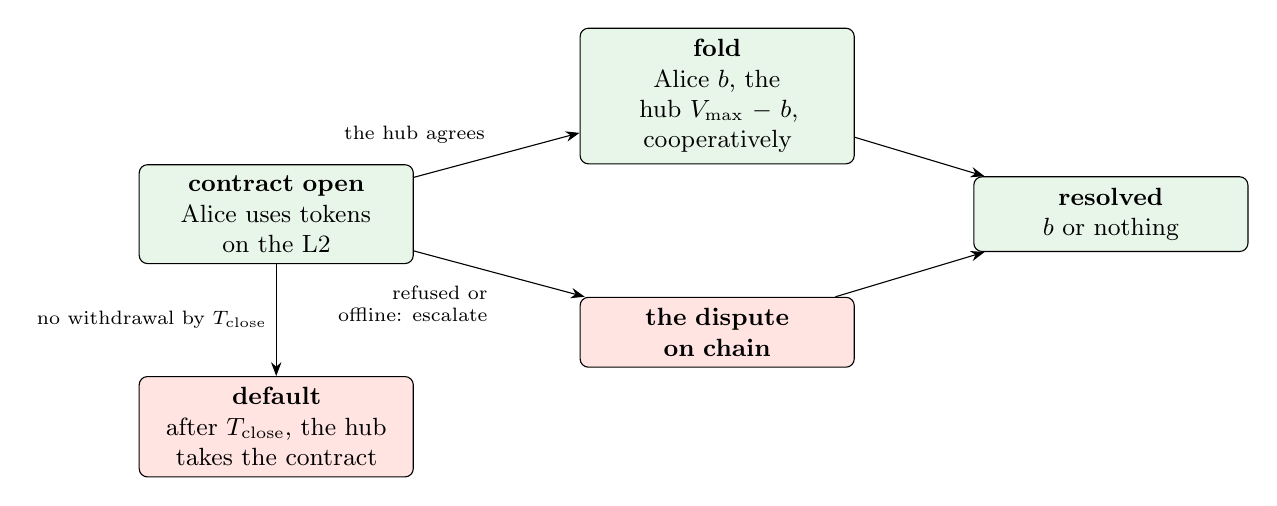
\begin{tikzpicture}[
  font=\small,
  st/.style={draw, rounded corners=3pt, align=center, inner sep=4pt, text width=#1},
  st/.default=32mm,
  >={Stealth[length=5pt]},
]
\node[st, fill=coop] (live) at (0,0) {\textbf{contract open}\\Alice uses tokens\\on the L2};
\node[st, fill=coop] (fold) at (5.6,1.5) {\textbf{fold}\\Alice $b$, the hub $\vmax - b$,\\cooperatively};
\node[st, fill=chainc] (ladder) at (5.6,-1.5) {\textbf{the dispute on chain}};
\node[st, fill=chainc] (def) at (0,-2.7) {\textbf{default}\\after $\Tc$, the hub\\takes the contract};
\node[st, fill=coop] (end) at (10.6,0) {\textbf{resolved}\\$b$ or nothing};
\draw[->] (live) -- node[above left=1pt, font=\scriptsize] {the hub agrees} (fold);
\draw[->] (live) -- node[below left=1pt, font=\scriptsize, align=right] {refused or\\offline: escalate} (ladder);
\draw[->] (live) -- node[left, font=\scriptsize] {no withdrawal by $\Tc$} (def);
\draw[->] (fold) -- (end);
\draw[->] (ladder) -- (end);
\end{tikzpicture}
\caption{The life of a contract. Green states stay off-chain or settle
cooperatively; red states are on chain.}
\label{fig:life}
\end{figure}

\section{How a withdrawal from the L2 is proved valid}
\label{sec:statement}

\subsection{The statement proved}

For brevity we have not yet given a description of what such an L2 must look like, but its main features are here, to explain the proof structure.

The L2 is a ledger of notes, with state updates signed by a sequencer\footnote{We'll talk more about achieving finality via Bitcoin or otherwise later~[\ref{sec:finality}].}. A note is an owner, a value, a memo and a
random $\rho$, which makes every note distinct (two equal payments to the
same owner are still two notes); its commitment is a SHA-256 hash of
these, and the commitments form an append-only Merkle tree. A spent note
is not removed from the tree, which would change every other note's
path, but recorded by its \emph{nullifier}, a hash of its commitment, in
a set the sequencer keeps: spending a note twice repeats its nullifier.
So a note's path under a root stays valid however the ledger moves on.
In case we want \emph{shielded} transactions, as implemented in ~\cite{lichencode}, $\rho$
also hides the note's contents, and the nullifier is derived from a
secret key so that nobody can link it to its note. A
state root SR hashes the height, the tree's root and the nullifier
set's root, and the L2's sequencer signs it (BIP340). 

With this context, we can understand what the withdrawal proof actually does. The user provides:

\begin{enumerate}
\item A note owned by the hub, of value b and memo c, marked as ``withdrawal'' is in the commitment tree of a state root SR. This is a Merkle path from the note to the root.

\item The sequencer published that root. SR carries the sequencer's signature, for its L2 height.
\item Validity back to genesis. A chain receipt (the sequencer's recursive proof) shows that every L2 block from genesis to now was a valid state transition. The same receipt covers anchoring: each anchor spends the previous anchor's output, starting from the L2's genesis seal. Each is in a real Bitcoin block, by Merkle path to that block's header. The last\footnote{See Section ~\ref{sec:finality}; this needn't be the last SR in time, but only a unique history, because (currently) we are using a special withdrawal transaction, not any arbitrary note} anchor committed exactly SR, at its height. So SR is the root of the one anchored history.
\item Finality. Bitcoin headers follow on from the anchor's block, each meeting its own difficulty target, with total work of at least W. W is fixed when the contract opens, about 10 blocks' worth.
\end{enumerate}

The result is the public output $b \,\|\, c \,\|\, \mathcal{D}$. $\mathcal{D}$ identifies the contract: the sequencer's and hub's keys, the genesis output and W. So a proof for another deployment, history or finality threshold is a proof of a different statement. Bitcoin reads b for the payout, and checks c and $\mathcal{D}$ against the contract's terms. Since the chain proof's program id is built into the withdrawal program, the one program id the contract pins covers both.

Not fully addressed yet, however:

\begin{itemize}
\item This is not (yet) a proof of heaviest chain; that would require a counter-proof mechanism. It's currently judged that building a 10 block fork is expensive enough to make attack uneconomic.
\item Sequencer going quiet, or censoring user transfers: it is planned to implement a counter-proof design, slightly different from the above, in which the prover proves owning the note, and the hub can counter-prove spentness, because in the current design, a dead sequencer loses the user's money at $\Tc$.
\item The data availability question has not been addressed.
\end{itemize}

\subsection{From a program to a verifiable claim}

\begin{figure}[H]
\centering
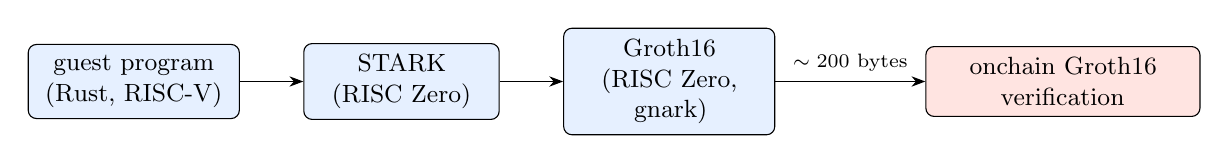
\begin{tikzpicture}[
  font=\small,
  box/.style={draw, rounded corners=3pt, align=center, inner sep=4pt, text width=#1},
  box/.default=27mm,
  >={Stealth[length=5pt]},
]
\node[box=24mm, fill=proofc] (g) at (0,0) {guest program\\(Rust, RISC-V)};
\node[box=22mm, fill=proofc] (s) at (3.4,0) {STARK\\(RISC Zero)};
\node[box=24mm, fill=proofc] (w) at (6.8,0) {Groth16\\(RISC Zero, gnark)};
\node[box=32mm, fill=chainc] (v) at (11.8,0) {onchain Groth16\\verification};
\draw[->] (g) -- (s);
\draw[->] (s) -- (w);
\draw[->] (w) -- node[above, font=\scriptsize] {$\sim200$ bytes} (v);
\end{tikzpicture}
\caption{The withdrawal statement runs in RISC Zero's zkVM; its proof is
compressed to a Groth16 proof; a dispute is over the execution of a fixed
RISC-V program that verifies it~\cite{risc0,bitvmx}. A companion note
explains each stage~\cite{pipeline}.}
\end{figure}

\paragraph{What the contract must bind.} Whatever gadget settles a
dispute, the contract must tie the disputed proof to three things: the
program, since a valid proof of another program proves nothing; this
contract's terms, its memo $c$ and identifier $\mathcal{D}$ (the deployment's keys,
the genesis seal and the work $W$), so that a proof for another contract,
deployment, history or finality threshold fails; and the amount $b$, in a
form Script can read, for the payout (Section~\ref{sec:outcomes}). With
RISC Zero, the proof's public input is a digest of the program's image id
and its journal $b \,\|\, c \,\|\, \mathcal{D}$; because RISC Zero's Groth16 key is
the same for every program, the image id must be checked explicitly (one
suffices, since the withdrawal program has the chain program's id built
in). How the binding is enforced is the gadget's business. Under BitVMX,
Alice signs the verifier's input word by word and the contract checks the
image id, $c$ and $\mathcal{D}$, and reads $b$, from those signatures
\cite[\S 2]{lichenbitvmx}. Under BABE, the image id, $c$ and $\mathcal{D}$ are fixed
when the contract is set up, and $b$, which cannot be, is bound by the
hub's signature on the amount Alice asserts \cite[\S 5]{lichenbabe}.



\section{Settling a dispute on Bitcoin}
\label{sec:blocks}

The contract is a single taproot output, 2-of-2 between Alice and the
hub, whose leaves hold the ways it can end; transactions pre-signed at
opening let either party carry out its side of a dispute without the
other. What settles a dispute is an on-chain \emph{verification gadget}.

The idea is, given a proof whose public input binds the
program's context ($b \,\|\, c \,\|\, \mathcal{D}$ as mentioned above), adjudicate the
claim on Bitcoin. The context is checked, the amount $b$ is read into Script, and the loser pays. To emphasize: this is all verification. The proving side, up to the Groth16 proof, is the same whichever gadget is used.

\subsection{Values that Script can read: one-time signatures}

Bitcoin Script can check a signature only on the spending transaction,
never on a message of the signer's choosing. A contract that must act on
a value a party chooses later, above all Alice's $b$, uses Winternitz
one-time signatures, which Script verifies by hashing alone, leaving the
signed digits on the stack to compare~\cite{bitvm,bitvmx}. The keys are
exchanged when the contract opens, one per value, each used once;
signing two different values under one key is \emph{equivocation},
which a leaf can prove, giving the signer's stake to its counterparty.
Every gadget below reads $b$ this way.

\subsection{Implemented: BitVMX}

BitVMX~\cite{bitvmx} settles a claim about a RISC-V program's run by an
interactive search over its execution. Alice claims that the Groth16
verifier, run on her signed input, halts with success; if the hub
disagrees, they narrow the run down, eight segments a round, to a single
step, which Alice then proves in Script or the hub disproves. Each move
is a pre-signed transaction carrying the mover's one-time signatures,
and a lie about a memory read is caught through an authenticated jump
list instead of a second search. It is built and has been played to the
end on Mutinynet; the companion paper~\cite{lichenbitvmx} gives the
transaction graph and the measurements.

\subsection{Designed: BABE with authenticated amounts}

BABE~\cite{babe} replaces the search with three transactions. At setup,
the hub garbles a small circuit that turns the first element of Alice's
proof into the key of a witness encryption, so that only a valid proof
unlocks the secret she needs to be paid. Its obstacle is that the
statement is fixed at setup, while Alice chooses $b$ only when she
withdraws. The amount therefore moves into the witness, together with
the hub's one-time signature on it, which the hub must give on chain for
exactly the amount Alice asserted, or lose by timeout. This is our
proposal~\cite{delving}. Unlike GOAT's cryptographic
alternative~\cite{goat}, in our proposal, BABE's cryptography is unchanged. A companion note~\cite{lichenbabe} gives the construction, a sketch of its security and cost estimates; it is not built.

\begin{table}[!htp]
\centering
\small
\begin{tabularx}{\linewidth}{>{\raggedright\arraybackslash}p{58mm}LL}
\toprule
& BitVMX (measured) & BABE (estimated) \\
\midrule
exit against a vanished hub & 23~kvB, 5 transactions & ${\sim}4$~kvB \\
a true claim refused, played to the end & ${\sim}120$~kvB, 23 transactions & ${\sim}31$~kvB, 6 \\
the worst case & ${\sim}200$~kvB (a lie about a read) & the same as above \\
pre-signed per contract & 141 transactions & ${\sim}9$ \\
setup per contract, beyond pre-signing & none & minutes; ${\sim}90$~MiB stored by the user \\
contracts a hub can hold, disputes lasting a week\textsuperscript{*} & 3,300 (8,350 with a window per move) & ${\sim}56{,}000$ \\
\bottomrule
\end{tabularx}
\caption{The two gadgets~\cite{lichenbitvmx,lichenbabe}.
\textsuperscript{*}Before congesting the chain becomes a profitable
attack: for $N$ contracts, every move due within a window of $w$ blocks
must fit in it, $N s \le w \cdot 1\,\mathrm{MvB}$~\cite{floodloot}, and
the dispute lasts the sum of its windows.}
\label{tab:gadgets}
\end{table}

\section{The contract logic}
\label{sec:contract}

\subsection{Three ways out}

A contract ends in one of three ways; its output carries three leaves (not including a revocation if inside a channel):
\begin{itemize}[leftmargin=1.5em]
\item the \emph{fold}: a cooperative update of the channel (Alice
  $b + r_A$, the hub $\vmax - b + r_H$), the normal case, nothing on
  chain;
\item \tx{default}: after $\Tc$, a transaction pre-signed at the
  contract's opening pays the hub $\vmax + r_H$ and returns Alice's
  reserve $r_A$. This is the liveness requirement on Alice: turn up at the end, i.e. it's a very low bar requirement; whereas the hub must always be ready to answer disputes.
\item \tx{escalate}: Alice's claim goes on chain as the first step of
  the dispute. This will almost never happen, because given Alice's proof, the hub can calculate $\sim$ immediately that he's guaranteed to lose (since Groth16 verification is fast), so just pays out cooperatively (\emph{fold} as above).
\end{itemize}

\paragraph{On its own, or in a channel?} A contract is a standalone
output, a 2-of-2 between Alice and the hub, opened by one on-chain
transaction and folded by another. This is the design as built, and the
one this paper assumes. The same output could sit in a Lightning channel
commitment, making the fold a channel update and letting deposits arrive
as Lightning payments, as earlier LN-GAP code demonstrates. But the
price is high. Every channel update re-signs the contract's pre-signed
transactions for both commitments (under BitVMX, 141 each); renewal,
though off chain, is still a new contract and, under BABE, a new setup;
and a channel's revoked states bring back the always-on watchtower that a
standalone contract avoids (Section~\ref{sec:watch}). We treat it as a
possible later optimisation, not part of the design.

\subsection{Outcomes}
\label{sec:outcomes}

The dispute only ever decides Alice's withdrawal: $b$ if her claim
stands, nothing if it fails; the rest of $\vmax$ goes to the hub. The reserves follow the dispute: the loser's goes to the winner, whether
it lost on the merits, by signing two values of $b$ (\tx{equiv\_b}), or
by not answering in time. A party the gadget rules against loses the
whole contract, reserves included, so a provable lie costs the liar
everything.

\paragraph{Paying $b$: the bit outputs.} When Alice wins, the payout
must send her $b$, a value she chose when she claimed; but the
payout is pre-signed, so its amounts are fixed, and Script cannot
compute an amount. One pre-signed transaction per possible $b$ would be
too many. Instead, as for numeric DLCs~\cite{dlcnumeric}, the payout decomposes
$b$ in binary. Amounts are counts of one satoshi, and a contract of $K$
bits has the cap $\vmax = 2^K - 1$~sats; the payout has one output of
$2^i$~sats for each bit $i$ from 9 to $K - 1$, each with three leaves:
\begin{center}
\small
\begin{tabular}{lll}
\toprule
leaf & spent by & condition \\
\midrule
Alice's & Alice, after a delay $\delta$ & her one-time signature on $b$ has bit $i$ set \\
the hub's & the hub & the same signature has bit $i$ clear \\
\tx{equiv\_b} & the hub & two signatures on different values of $b$ \\
\bottomrule
\end{tabular}
\end{center}
Since $b$ is under a one-time key, the bits Alice can claim are those of
the single value she signed, and their outputs sum to $b$; the hub takes
the rest. Bits below 9 have no output, so a withdrawal settled by
dispute is paid in multiples of 512~sats, the remainder going to the
hub. For $b = 5{,}120$~sats she takes the outputs for bits 10 and 12.
Her leaves wait $\delta$ so that the hub can show an equivocation first.
A contract of $K = 24$ bits has a cap of about 0.168~BTC and 15 bit
outputs; each output's spend is about 330~vB, and each party can sweep
its outputs in one transaction. The reserves sit in one more output,
paid to the winner, with an \tx{equiv\_b} leaf of its own. In the
cooperative fold none of this appears: the fold simply pays $b$.

\paragraph{The contract reserve.} As in Lightning, a penalty deters only
a party with something to lose, and here that is not what each party put
in but what each loses by losing a dispute. Alice risks only her honest
outcome, the return she could actually prove, which is nothing once she
has spent her tokens: a false claim of $\vmax$ is then a free option on
the hub being offline. The hub makes no claims, only refusals, and
losing a dispute costs it only fees, so it can refuse a valid withdrawal
and hope Alice cannot play her side in time. Hence a reserve on each
side, moved only by a lost dispute. A probe that succeeds with chance
$p$ gains up to $\vmax - b$ and otherwise costs the reserve, so it is
unprofitable when
\[
  (1-p)\, r_A > p\,(\vmax - b), \quad\text{that is, for every } p < \frac{m}{1+m} \text{ with } r_A = m\,(\vmax - b).
\]
At $m = 1\%$, the size of a Lightning channel reserve, that deters only
probes with less than a 1\% chance; at $m = 1$, those with less than even
odds. Where to sit on that curve depends on what the parties know of
each other. In any case, a lost dispute should cost the loser at least
the other side's fees. Part of those is known when the contract is
signed: the fee floors of its pre-signed transactions, 197,356~sats in
the deepest dispute under BitVMX~\cite[\S 6]{lichenbitvmx}. So neither
reserve should be smaller, and lichen's hub takes for its own the larger
of its share of the cap and that figure.

\paragraph{Who it suits.} A reserve is locked, not spent: an honest
party loses it only by losing a dispute, which for an honest Alice means
going absent in the middle of one. The binding cost falls on the hub,
whose reserve must cover Alice's worst-case dispute however small her
balance. Under BitVMX that is about 117~kvB, 117,000~sats at 1~sat/vB
and 1.2 million at 10, so the contract suits balances from about half a
million sats; under BABE, about 12.5~kvB (estimated), so balances of some
tens of thousands. Large balances add no cost: the dispute does not grow
with $b$. Amounts are 32-bit counts of one satoshi, so a contract holds
up to about 42.9~BTC.

\subsection{User liveness and watchtowers}
\label{sec:watch}

The user needs to be online at two times only: before $\Tc$, to withdraw or
renew, and during a dispute, which only she can start. How demanding the
dispute is depends on the gadget. Under BitVMX it is a dozen moves over
hours (days on mainnet), each due within a window, and each is her
one-time signature on values that depend on the hub's last move, so they
cannot be signed in advance and handed to a watchtower, as Lightning's
penalty transactions are. Under BABE she has one move under time
pressure, a few hundred bytes, after which she can withdraw at leisure.

Because a standalone contract gives the hub nothing to broadcast against
her, Alice can delegate in a way Lightning cannot: to a \emph{tower} of
her own, started only when a withdrawal is refused and discarded after.
It holds her contract's pre-signed transactions and the keys for her
moves, but not the key to her amount, so it can play her side, and at
worst play it badly, but cannot claim a different amount. Lichen's tower
does this, proving the withdrawal and playing a hostile hub to the payout
on Mutinynet in about 75 minutes~\cite[\S 10]{lichenbitvmx}. Embedding
the contract in a Lightning channel gives this up: a channel's revoked
states bring back the need for an always-on watchtower.

\section{Finality from Bitcoin}
\label{sec:finality}

With a single, or indeed a distributed, sequencer signing updates to L2 state, without a consensus mechanism like proof of work or proof of stake, it's free to ``rewrite history'' for transactions on the L2, enabling double spend attacks. The techniques used in ETH L2s to handle this involve the rollup data publication and contract state on the base chain; that is not available here. So in the absence of proposing expensive consensus on L2, it makes the most sense to inherit finality from Bitcoin, as Shielded CSV~\cite{shieldedcsv} and Shielded Bitcoin~\cite{shieldedbtc} do (the first by publishing each transaction's nullifier on Bitcoin, the second by publishing every transaction there in full), but here using the single use seal concept~\cite{toddseals}, with one commitment per batch.

If each sealed batch's root is committed in a Bitcoin transaction that spends the previous batch's commitment output, a fork of the layer 2 needs a double spend on Bitcoin. It costs one small transaction per batch, not per layer 2 transaction. A committee of sequencers then needs only one honest member for inclusion (members append batches in turn); forks are excluded by Bitcoin, not by a threshold.

What sealing does not provide is availability: a seal commits to a root, not to the data behind it. This paper \underline{does not} answer this question; it is a function of exactly how the L2 ledger is constructed (with a Bitcoin publication component, or not). But if data availability is not addressed, the user does have to trust the sequencer in a very concrete sense: if the sequencer refuses to provide the Merkle path for her return note, the user has no way to retrieve their funds in the contract, and loses them. This strongly argues for the above-mentioned ``committee of sequencers'', because you just need 1 to include your withdrawal and give you its path to be safe\footnote{A more advanced idea is publishing withdrawals on Bitcoin, requiring L2 to read L1 in a similar way to what is described next}.

\paragraph{What the withdrawal statement checks.} The sequencer's
anchors form one chain of spends on Bitcoin: each spends the output the
previous one created, starting from the layer 2's \emph{genesis seal},
and commits to the history of state roots up to its height. Each anchor
is recorded on L2, and the chain proof
checks it with the rest: that its transaction spends the previous seal, and
that it sits in the block it names, by a Merkle path to that block's
header. 
When Alice withdraws (in the currently implemented design) she provides a root that has been anchored (not necessarily the most recent) along with a withdrawal transaction she performed, which is sufficient for proof, because the anchors provide a unique history (there is no other history, we claim, where she keeps the money on L2 while withdrawing).

The withdrawal
statement also requires that Bitcoin headers follow the anchor's block, each
linking to the one before and meeting its own difficulty target, with
total work at least $W$. The genesis seal and $W$ are part of the
contract's identifier $\mathcal{D}$, so the contract fixes both: $W$
is set when the contract opens, as ten blocks' work at the difficulty of
that moment. A header declares its own difficulty, but that gains a
forger nothing: work is summed, and producing headers worth $W$ in total
costs about $W$ hashes however the difficulty is split among them. So
no retarget rule needs checking, and the contract's length does not
matter.

\paragraph{The cost is small.} About ten headers, each two or three
SHA-256 compressions, which RISC Zero accelerates: a few thousand cycles
of a withdrawal statement that costs 389,020 cycles in all. For the
sequencer, the chain proof's check of an anchor record is about 135,000
cycles. The dispute is unchanged. In the cooperative case, the hub
checks the anchors with its own node.

Forgery then becomes a matter of mining a fork in Bitcoin itself. In current Bridge designs, like Union~\cite{union}, a challenger answers the claimant's chain with a
heavier one, which the claimant may dispute in turn, in a second BitVMX
game with the roles reversed.

But we don't want to or need to do that; the claimant is always the user and the dispute is settled on one statement.

So any forgery attack is on the side of the user; and such an attack to achieve maximum returns \emph{could} use it to steal from the hub across multiple contracts.
So the bound is not one contract's cap but
the hub's total headroom exposed to a single forged chain. As long as
that stays well below the reward of the blocks a fork must replace, the attack remains un-economic. This is the kind of security you can claim for Bitcoin itself, basically.

\section{Scaling with multiple hubs}
\label{sec:multihub}

The worst failure mode for a Lichen-style L2 is \underline{mass exit}. As we know even in Lightning there is the idea that, if the number of users is high enough, mass publication of old/invalid states could lead to an excessive reliance on prompt confirmation on a blockchain where space is a scarce resource.

Now imagine lichen similarly, but with that problem exacerbated: a hub holding 60,000 users (note: the problem is not \emph{necessarily} any better with the 60k spread over multiple hubs). Now each withdrawal may take a number of transactions and a chunk of vB, with the numbers depending on the verifier gadget used. It's clearly the case that a malicious hub can trigger a very large block space demand and, with a lot of difficulty to be fair, \emph{could} steal from many honest users at once depending on the order in which transactions get confirmed. The same attack exists in reverse: if a user-attack generates a ton of Sybil contracts with one hub, they could trigger mass exit with fraudulent exit requests.

It is worth mentioning that the more likely failure mode --- that is of hub infrastructure failure leading to offlineness --- tends to use up less onchain space with any verifier gadget used for the onchain transactions, but it can still be quite significant, even here.

Two things must be chosen to get a sense of the potential safe scale of a Lichen L2: how long is the dispute phase allowed to last? And, how much fees must be held in reserve by both parties to ensure that the dispute can fully play out in time? Given this data, some specific, though estimated, numbers of how many users a hub can support, can be generated. These numbers are laid out in~\cite{lichenbitvmx} and~\cite{lichenbabe}.

We can improve these figures on \emph{some} axes by having multiple hubs. If we had 20 distinct hubs of 3000 users and not 1 hub of 60,000 it would reduce some risk for users in particular. Which leads to the question:

\paragraph{ Can you pay users in a different hub?} Certainly you can, with some infrastructure. There's more than one way to do it, but for brevity we describe the simplest: if Hub 1 and Hub 2 exist, with their own distinct ledgers, Alice on Hub 1 can pay Bob on Hub 2, in bitcoin, if Hub 2 has a contract on Hub 1 with inbound capacity. She simply pays Hub2's address on Hub 1's ledger, contingent on an atomic swap set up with the payment to Bob on Hub 2's ledger. There could also be routing, but the principle is clear.

\paragraph{Different ledgers?} It seems natural in this multi-hub world to allow users to use a Hub whose ledger rules (e.g. does it use shielded transactions or smart contracts or ..) can be distinct and whose consensus establishing mechanisms are distinct. Alternatively they could all rely on the same finality and proof of validity, in one ledger, as distinct assets.

\section{Costs}
\label{sec:costs}

Many costs will be specific to the verifier gadget chosen, so we point the reader at~\cite{lichenbitvmx} and~\cite{lichenbabe}. However some costs come from the generic Risc0 architecture chosen:

\paragraph{Can a user dispute on her own hardware?} A dispute needs
a non-urgent (only $\Tc$ bounds
a withdrawal) but non-trivial computation from Alice (though nothing is needed in the cooperative case, where the hub
reads the layer 2 directly). That is, a proof of her withdrawal. As built,
the statement costs 389,020 zkVM cycles, one segment, using RISC Zero's
accelerators (about 10 cycles for a 256-bit modular multiplication, 68
for a SHA-256 block~\cite{risc0accel}); without them it was 5.9
million, almost all of them in the sequencer's signature. Proving it
takes 74~s on an Apple M4 Pro and 359~s on a
4-vCPU x86 server, which smaller
segments reduce~\cite{risc0data}; a CUDA GPU would be faster still. The Groth16 wrap is a fixed cost of a few minutes with 8~GB of memory at peak, today on x86
only; it can be delegated, since the wrapper sees only the receipt and
its public journal. A phone is plausible for the proof with small segments and a delegated wrap.

\paragraph{Onchain costs} For the anchoring of L2 state updates, there is an anchor per batch, 269 vB, including the OP\_RETURN output for SR. For each individual contract, a fold costs 193 vB. Even for faster L2s with more aggressive finality, a cost of 269 vB every block or few blocks is trivial.

\section{Positioning}
\label{sec:positioning}

We have already briefly discussed how this is different from just ``payments over Lightning via a hub'' in the Introduction. We'll list here some key differences to some other existing L2 or L2-like Bitcoin constructions.

\paragraph{Against BitVM2 and Union.} We consider BitVM2~\cite{bitvm2usenix}, and
Union~\cite{union}, a bridge to Rootstock built on BitVMX by BitVMX's
own authors. Both release bitcoin on Bitcoin against a claim about
a program's execution, settled by fraud proof, with no change to
consensus, and, like lichen, inherit the assumptions of a side system they
do not secure. They differ in who the parties are, and most of the rest
follows (Table~\ref{tab:bitvm2}).

\begin{table}[!tp]
\centering
\small
\begin{tabularx}{\linewidth}{>{\raggedright\arraybackslash}p{21mm}LLL}
\toprule
& a BitVM2 bridge & Union & lichen \\
\midrule
custody & one pool for all users & one pool, in fixed-size outputs, one per peg-in & a contract for each user, with the hub \\
pre-signed by & a committee, for every operator's graph on every deposit & the $N$ functionaries, a two-party game for every pair of them on every peg-in & the user and the hub \\
setup trust & one honest committee member & one honest functionary & none \\
the claimant & an operator, who paid the user from its own funds and claims reimbursement & a functionary, likewise & the user, for her own withdrawal \\
the challengers & anyone; safety needs one honest one watching & the other functionaries; safety needs one honest one watching & the hub alone, the only party a false claim can rob \\
the dispute & one round: the operator asserts the verifier's intermediate values, a challenger reveals one failing chunk (scripts up to 4~MB); 42 blocks & BitVMX's interactive search, 4-ary: about 270~kvB at worst; a heavier chain is answered in a nested game & Depends on verification gadget \\
the user's part in a dispute & none: she was paid up front & none, likewise & a party: she plays her side, or her tower does \\
a refused withdrawal & it waits for a willing operator & it waits for a willing functionary & she enforces it on chain herself \\
stakes & operators' collateral; challengers fund the assert & bonds sized to dispute costs, shared by a packet of peg-ins & the contract reserves $r_A, r_H$ \\
liquidity & operators front withdrawals until reimbursed & functionaries likewise, one peg-out each at a time & the hub locks $\vmax - D + r_H$ for each user until $\Tc$ \\
the asset & bridged bitcoin, fixed amounts & bridged bitcoin, fixed amounts & variable amount bitcoin within each user's cap, credit beyond it \\
expiry & none & none & $\Tc$: withdraw, or renew, before it \\
\bottomrule
\end{tabularx}
\caption{Two bridges and lichen. The bridges' figures are their
authors' estimates; lichen's depend on the gadget; see~\cite{lichenbitvmx},~\cite{lichenbabe} for measurements and estimates.}
\label{tab:bitvm2}
\end{table}

The bridges pool their users' bitcoin, and a pool shared by users not
yet known must be released by transactions that someone signs in
advance on their behalf: BitVM2's committee, Union's functionaries.
What then shapes the dispute is who may challenge a false claim. BitVM2
opens challenge to anyone, since anyone might be the one robbed; with
the challengers unknown when the graph is signed, no interactive game
can be pre-signed with them, so its dispute is a single round, in which
the operator puts the verifier's whole intermediate state on chain at
once. Union closes challenge to its functionaries, who are known at
setup, and so can pre-sign BitVMX's interactive search between every
pair of them, which puts less data on chain over many more rounds. Its
price is that safety needs an honest functionary not only at setup but
online whenever a claim is made, and that the pairwise games, and the
bonds that fund them, grow with the number of functionaries. A lichen
contract is not pooled: it has two parties, both present when it opens.
They pre-sign it themselves, so there is no committee and no setup
trust; only the hub can be robbed by a false claim, so only the hub
challenges; and the search between them is Union's game with a single
pair. Splitting the pool has its own price: the hub's locked liquidity,
a token that is bitcoin only within each user's cap, an expiry, and a
user who must take part in her own dispute. \textbf{The bridges ask their users
to trust one signer at setup and one challenger afterwards, and to be
present for none of it; lichen asks them to trust no one, but to be
present for their own disputes}.

\paragraph{Other designs, briefly.}
\begin{itemize}[leftmargin=1.5em]
\item \emph{Ecash} (Cashu, Fedimint): lichen removes the mint's power to
  take the funds, within each user's cap, at the price of the hub's
  locked liquidity; the mint may print as it likes, but every redemption
  is against its own collateral.
\item \emph{Ark}: a shared tree of outputs with an operator and an
  expiry, where a lichen contract is per user; both ask users to act
  before an expiry. An Ark balance is a claim on a specific pre-signed
  output, exitable by its holder alone; a lichen balance is held in sats
  on a programmable ledger and redeemed one-for-one in bitcoin from the
  hub's collateral, without the hub's cooperation, up to the holder's
  contract cap, and is credit on the hub beyond it.
\item \emph{Payment pools} (one shared output, balances updated by all
  members): need every member's signature for an update and a covenant
  (or an exponential tree) for unilateral exit; a lichen transfer needs
  only its sender, and exit needs no consensus change.
\end{itemize}

\section{Implementation}
\label{sec:status}

The design is implemented in proof-of-concept form as two code bases, LN-GAP~\cite{lngapcode} and Lichen~\cite{lichencode}, with tests and demos executed on bitcoin regtest and on mutinynet. Any bitcoin-related data in this paper come from the concrete executions there, including playing out disputes fully.

The implementation uses the BitVMX gadget~\cite{lichenbitvmx} and a shielded-notes L2 for private offchain transfers. Validity proofs are implemented, along with anchors in bitcoin transactions for finality.

Some features are not yet in place, though: in particular, there is not currently a way for the user to exit when the sequencer dies or censors. This should be addressable, as has been noted, with a counter-proof mechanism for the hub, a slight design change. Additionally, though the BABE variant has been theorized as a definite upgrade in scalability, it has not yet been coded.

\begin{thebibliography}{99}

\bibitem{lngap} waxwing. LN-GAP: Lightning governed by arbitrary programs. Version 1.0 (draft), September 2026. \url{https://github.com/AdamISZ/ln-gap/blob/master/docs/paper/lngap_draft.pdf}

\bibitem{pipeline} waxwing. From a Rust program to one step on Bitcoin: how a withdrawal is proved, wrapped and disputed in LN-GAP 2.5. October 2026. \url{https://github.com/AdamISZ/ln-gap/blob/master/docs/paper/pipeline.pdf}

\bibitem{lichenbitvmx} waxwing. Lichen over BitVMX: the dispute, as built and measured. Version 0.1, October 2026. \url{https://github.com/AdamISZ/lichen/blob/master/papers/lichen-bitvmx-v0.1.1.pdf}

\bibitem{lichenbabe} waxwing. Lichen over BABE: withdrawals of a variable amount, by authenticated request. Version 0.1, October 2026. \url{https://github.com/AdamISZ/lichen/blob/master/papers/lichen-babe-v0.1.1.pdf}

\bibitem{babe} S.~Garg, D.~Kolonelos, M.~Sergeevitch, S.~Sridhar and D.~Tse. BABE: verifying proofs on Bitcoin made 1000x cheaper. ePrint 2026/065, revised October 2026. \url{https://eprint.iacr.org/2026/065}

\bibitem{goat} GOAT Network research. Dynamic public inputs in BABE (deferred binding). HackMD, 2026. \url{https://hackmd.io/@goatresearch/B1N9g2uOee}

\bibitem{delving} waxwing. Variable payout amounts for BABE, as applied to Lichen. Delving Bitcoin, October 2026. \url{https://delvingbitcoin.org/t/variable-payout-amounts-for-babe-as-applied-to-lichen/2963}

\bibitem{lngapcode} LN-GAP proof-of-concept code. \url{https://github.com/AdamISZ/ln-gap}

\bibitem{lichencode} lichen: the ledger, the sequencer, the hub and the wallet. \url{https://github.com/AdamISZ/lichen}

\bibitem{bitvmx} S.~D.~Lerner, R.~Amela, S.~Mishra, M.~Jonas and J.~\'Alvarez Cid-Fuentes. BitVMX: a CPU for universal computation on Bitcoin, 2024. \url{https://arxiv.org/abs/2405.06842}

\bibitem{bitvmxcpu} FairgateLabs. BitVMX-CPU: the emulator, the $n$-ary search and the Groth16 verifier for BitVMX. \url{https://github.com/FairgateLabs/BitVMX-CPU}
\bibitem{bitvmxfork} BitVMX-CPU with LN-GAP's changes (two bug fixes, the authenticated jump list), branch \texttt{lngap}. \url{https://github.com/AdamISZ/BitVMX-CPU}

\bibitem{lightning} J.~Poon and T.~Dryja. The Bitcoin Lightning Network: scalable off-chain instant payments, 2016. \url{https://lightning.network/lightning-network-paper.pdf}

\bibitem{bitvm} R.~Linus. BitVM: compute anything on Bitcoin, 2023. \url{https://bitvm.org/bitvm.pdf}

\bibitem{bitvm2usenix} R.~Linus Woll, L.~Aumayr, Z.~Avarikioti, M.~Maffei, A.~Pelosi, O.~S.~Thyfronitis Litos, C.~Stefo, D.~Tse and A.~Zamyatin. Bridging Bitcoin to second layers via BitVM2. USENIX Security 2026; ePrint 2025/1158. \url{https://eprint.iacr.org/2025/1158}

\bibitem{union} R.~Amela, S.~Mishra, S.~D.~Lerner and J.~\'Alvarez Cid-Fuentes. Union: a trust-minimized bridge for Rootstock, 2025. \url{https://arxiv.org/abs/2501.07435}

\bibitem{risc0} RISC Zero. The RISC Zero zkVM and its Groth16 receipts. \url{https://dev.risczero.com}

\bibitem{bitvmxinnov} S.~D.~Lerner. Latest innovations in BitVMX (trace Merkle tree, authenticated skiplist and jumplist), June 2024. \url{https://bitvmx.org/knowledge/latest-innovations-in-bitvmx}

\bibitem{floodloot} J.~Harris and A.~Zohar. Flood \& Loot: a systemic attack on the Lightning Network. AFT 2020. \url{https://arxiv.org/abs/2006.08513}

\bibitem{toddseals} P.~Todd. Preventing consensus fraud with commitments and single-use-seals, 2016. \url{https://petertodd.org/2016/commitments-and-single-use-seals}

\bibitem{risc0accel} RISC Zero. Cryptography acceleration (SHA-256 and 256-bit modular multiplication circuits; patched \texttt{k256}, \texttt{sha2}). \url{https://dev.risczero.com/api/zkvm/acceleration}

\bibitem{risc0data} RISC Zero. zkVM datasheet: proving time and memory by cycle count, CPU, Metal and CUDA, April 2023. \url{https://dev.risczero.com/datasheet.pdf}

\bibitem{dlcnumeric} DLC specifications: numeric outcome compression. \url{https://github.com/discreetlogcontracts/dlcspecs}

\bibitem{shieldedcsv} J.~Nick, L.~Eagen and R.~Linus. Shielded CSV: private and efficient client-side validation. ePrint 2025/068. \url{https://eprint.iacr.org/2025/068}

\bibitem{shieldedbtc} C.~Shikhelman, M.~Komarov and A.~Moskvin. Shielded Bitcoin: private transfers on the Bitcoin L1. [alloc] init, September 2026. \url{https://www.allocinit.xyz/uploads/shielded-bitcoin.pdf}

\end{thebibliography}

\end{document}
